\documentclass{article}[12pt]
\usepackage{fullpage}
% Packages
\usepackage{amsfonts}
\usepackage{amsmath}
\usepackage{amsthm}
\usepackage{graphicx}


%\theoremstyle{plain}
\usepackage{amsmath,bm}

\newtheorem{lemma}{Lemma}
\newtheorem{claim}[lemma]{Claim}
\newtheorem{theorem}[lemma]{Theorem}
\newtheorem{corollary}[lemma]{Corollary}
\newtheorem{definition}{Definition}
\newtheorem{question}{Question}

\newcommand{\note}[1]{\par{\bf Note:}#1\par}
\newcommand{\notem}[1]{{\marginpar{\tiny #1}}}

\newcommand{\figline}{\rule{\textwidth}{1pt}}

%\newcommand{\proof}{\noindent{\bf Proof:} }
%\newcommand{\qed}{\rule{0.7em}{0.7em}}

\newcommand{\newmcommand}[2]{\newcommand{#1}{{\ifmmode {#2}\else\mbox{${#2}$}\fi}}}
\newcommand{\newmcommandi}[2]{\newcommand{#1}[1]{{\ifmmode {#2}\else\mbox{${#2}$}\fi}}}
\newcommand{\newmcommandii}[2]{\newcommand{#1}[2]{{\ifmmode {#2}\else\mbox{${#2}$}\fi}}}
\newcommand{\newmcommandiii}[2]{\newcommand{#1}[3]{{\ifmmode {#2}\else\mbox{${#2}$}\fi}}}

\newcommand{\E}[2]{{\bf E}_{#1}\left[ #2 \right]}
%\newcommand{\D}[2]{{\bf D}_{#1}\left[ #2 \right]}
\newcommand{\D}{{\cal D}}

\renewcommand{\P}[2]{{\bf P}_{#1}\left[ #2 \right]}
\newcommand{\reals}{\mathbb{R}}

\newcommand{\argmin}{\mbox{argmin}}
\newcommand{\argmax}{\mbox{argmax}}
\newcommand{\SP}[1]{{\cal P}^{#1}} % strictly positive function of
                                   % order i
\newcommand{\R}{R}      % Cumulative regret
\newcommand{\vR}{\mathbf{R}} %regret vector

\renewcommand{\r}{r}      % Instantaneuous regret
\newcommand{\state}{{\bf \Psi}}
\newcommand{\1}[1]{{\mathbf 1}\left[#1\right]} % point mass at #1

\newcommand{\pot}{\phi}
\newcommand{\potPQ}{\pot_{\learnerM,\adversM}}
\newcommand{\potLA}{\pot_{\l,\a}}
\newcommand{\finalPot}[1]{\pmb{\phi}_{#1}}
\newcommand{\finalPotT}{\finalPot{T}}
\newcommand{\finalPotR}{\finalPot{\realT}}
\newcommand{\upperpot}{\pot_{\learnerM}^{\downarrow}}
\newcommand{\upperpotb}{\pot_{\learnerMb}^{\downarrow}}
\newcommand{\upperpotd}{\pot_{\learnerMd}^{\downarrow}}
%\newcommand{\upperpotj}{\pot_{\learnerM(j)}^{\downarrow}}
\newcommand{\upperpotMdk}{\pot_{\learnerMdk}^{\downarrow}}
\newcommand{\upperpotMdj}{\pot_{\learnerMdj}^{\downarrow}}


\newcommand{\lowerpot}{\pot_{\adversM}^{\uparrow}}
\newcommand{\lowerpotb}{\pot_{\adversMb}^{\uparrow}}
\newcommand{\lowerpotd}{\pot_{\adversMd}^{\uparrow}}
\newcommand{\lowerpotj}{\pot_{\adversM(j)}^{\uparrow}}
\newcommand{\lowerpotMdk}{\pot_{\adversMdk}^{\uparrow}}
\newcommand{\lowerpoteven}{\lowerpot_{\evensplit}}

\newcommand{\realT}{\mathcal{T}}  % the final time for the real-time
% game
\newcommand{\Tset}[1]{\pmb{T}_{#1}}
\newcommand{\Ilat}[1]{\pmb{I}_{#1}}
\newcommand{\Klat}[1]{\pmb{K}_{#1}}
\newcommand{\score}{\Phi}
\newcommand{\upperscore}[1]{\score_{#1}^{\downarrow}}
\newcommand{\lowerscore}[1]{\score_{#1}^{\uparrow}}

\newcommand{\upperscoreM}{\upperscore{\learnerM}}
\newcommand{\upperscoreMd}{\upperscore{\learnerMd}}
\newcommand{\upperscoreMdk}{\upperscore{\learnerMdk}}

\newcommand{\lowerscoreM}{\lowerscore{\adversM}}
\newcommand{\lowerscoreMd}{\lowerscore{\adversMd}}
\newcommand{\learnerM}{P}
\newcommand{\learnerMb}{P_I}
\newcommand{\learnerMd}{P_D}
\renewcommand{\l}{\learnerM}
\newcommand{\learnerMdk}{P_{D(k)}}
\newcommand{\learnerMdj}{P_{D(j)}}


\newcommand{\legalLearner}{{\cal L}}

\newcommand{\adversM}{Q}
\newcommand{\adversMb}{Q_I}  %Integer time game
\newcommand{\adversMd}{Q_D}  % Discrete time game
\newcommand{\adversMdk}{Q_{D(k)}}  %Discrete time game with step of
                                %size 2^{-k}


% \renewcommand{\a}{\adversM}
%\newcommand{\legalAdversary}{{\cal A}}
\newcommand{\agloss}{v}
\newcommand{\Bias}{B}
\newcommand{\deltat}{\Delta t}

\newcommand{\diffweight}{\l^d}   % learner strategy based on taking a difference
\newcommand{\upperpotdiff}{\upperpot_{\diffweight}}


\newcommand{\Binom}{\mathbb{B}}
\newcommand{\radsum}{\Binom(s_1,\ldots,s_T)}
\newcommand{\var}{\mbox{Var}}
\newcommand{\V}{V}


\newcommand{\at}[1]{\left\{ \left. #1
    \right|_{\begin{tiny}\begin{matrix}
          \tau,\rho=\\t_i,\R \end{matrix} \end{tiny}}
    \pot(\tau,\rho)\right\}}
\newcommand{\att}[1]{\left\{ \left. #1  
\right|_{\begin{tiny}\begin{matrix} \tau,\rho=\\t_i+g \deltat_i,\R_i+g
      r_i \end{matrix} \end{tiny}}
\pot(\tau, \rho)\right\}}


\newcommand{\atI}[1]{\left\{ \left. #1  
\right|_{\begin{tiny}\begin{matrix}
      x,y=\\x_0,y_0 \end{matrix} \end{tiny}}
f(x,y) \right\}}
\newcommand{\atII}[1]{\left\{ \left. #1
\right|_{\begin{tiny}\begin{matrix}
      x,y=\\x_0+t\Dx,y_0+t\Dy \end{matrix} \end{tiny}}
f(x,y) \right\}}


\newmcommandi{\paren}{\left({#1}\right)}
\newmcommandi{\brac}{\left[{#1}\right]}




\title{Potential-based hedging algorithms}
\author{Yoav Freund}
\begin{document}

\maketitle
\begin{abstract}
We study regret-minimizing online algorithms based on potential
functions. First, we show that any algorithm with a regret bound that
holds for any $\epsilon$ is equivalent to a potential minimizing
algorithm and vice versa. Second we should a min-max learning
algorithm for known horizon. We show a regret bound that is close to
optimal when the horizon is not known. Finally we give bounds on the
learning algorithm in the context of Ito processes.
\end{abstract}

\section{Introduction}

Online prediction with expert advise has been studied extensively over
the years and the number of publications in the area is vast (see
e.g.~\cite{vovk1990aggregating, feder1992universal,
  littlestone1994weighted, cesa1997use, cesa2006prediction}.

Here we focus on a simple variant of online prediction with expert
advice called {\em the decision-theoretic online learning game}
(DTOL)~\cite{freund1997decision}, we  consider the {\em
  signed} version of the online game.

DTOL is a repeated zero sum game between a {\em learner} and an {\em
  adversary}. The adversary controls the losses of $N$ actions, while
the learner controls a distribution over the actions.

\begin{figure}[ht!]
\framebox{
\begin{minipage}[t]{6.4in}
{\bf Decision theoretic online learning}\\~\\
For $t=1,\ldots,T$
\begin{enumerate}
    \item The learner chooses a weight function $w_j^t$ over the
      actions $j \in \{1,\ldots,N\}$. 
    \item The adversary chooses an {\em instantaneous loss} for each
      of the $N$ actions: \\
      $l_j^t \in [-1,+1]$ for $j \in \{1,\ldots,N\}$.
    \item The {\em cumulative loss of action $j$} at time $0 \leq t \leq T$
    is  $L^t_j = \sum_{s=1}^t l_j^s$. 
    \item The learner incurs an {\em instantanous average loss} defined as
      $\ell^t = \frac{\sum_{j=1}^N w_j^t l_j^t}{\sum_{j=1}^N w_j^t}$
    \item The {\em cumulative loss of the learner} is
      $L_\ell^t = \sum_{s=1}^t \ell^s$
    \item The {\em cumulative regret} of the learner with respect to action $j$ is $\R_j^t = L_\ell^t -L_j^t $.
\end{enumerate}
\end{minipage}}
\end{figure}


The goal of the learner is to perform almost as well as the best
actions. Specifically, we sort the regrets in decreasing order $\R_1^t \geq
\R_2^t \geq \cdots \geq \R_k^t \geq \cdots$ and define $\R_k^t$ to
as the regret relative to the $\epsilon=k/M$ top percentile, denote $\R_\epsilon^t$. Our goal
is to find algorithms that guarantee small upper bounds on
$\R_\epsilon^t$. Known bounds have the form $c \sqrt{t \ln
  {1/\epsilon}}$, but the algorithm has to be tuned based on prior
knowledge of $\epsilon$. We seek algorithms with regret bounds that hold {\em simultanously} for all values
of $\epsilon$. In other words algorithms that do not need to know
$\epsilon$ or $t$ ahead of time.

Formally, we say that the distribution over regrets $\state$ satisfied a
simultanous bound $B$ if
\begin{definition}[Simultanous regret
  bound] \label{def:unif-regret-bound} Let $G: \reals \to [0,1]$ be a
  non-increasing function which maps regret bounds to probabilities.
  A distribution over regrets $\state$ is simultanously bound by $G$ if
  \[
    \forall r \in \reals \;\; \P{\rho \sim \state(T)}{\rho \geq r} \leq G(r)
  \]
\end{definition}

A potential function is an increasing function
$\pot:\reals \to \reals$. Potential based learing algorithm
are designed to bound the the average potential:
%$\E{\R \sim \state}{\pot(\R)}$.  
\begin{definition}[Average potential bound] \label{def:aver-potential-bound}
  A distribution over he reals $\state$ satisfies the average
  potential function $\pot$ if
  $$\E{\R \sim \state}{\pot(\R)} \leq 1$$
  Where $\pot: \reals \to \reals^+$ is a non decreasing function. 
\end{definition}

We next show that there is a one to one relationship between
simultanous bounds and average potential bounds. 
\begin{theorem}\label{thm:simulBoundAveragePot}
 A distribution $\state$ is simultanously bounded by $B$ if and only
 if it satisfies the average potential bound with $\phi(\R) = B(\R)^{-1}$
\end{theorem}
Theorem~\ref{thm:simulBoundAveragePot} allows us to focus on potential
based algorithms.

As will be explained in Section~\ref{sec:potentials} potential
functions can be computed by backwards recursion. In other words,
given $\pot_T(R)$ and fixing the strategies for both learner and
adversary we can define a potential function $\pot_{T-1}(R)$ so that
the average potentials are equal:
\[
  \E{\R \sim \state(T-1)}{\pot_{T-1}(\R)} = \E{\R \sim \state(T)}{\pot_T(\R)}
  \]
  We use this equality to compare different strategies for both players.

We are interesting in proving min-max optimal bounds. However, as we
will show, there are no matching min-max strategies for the original
DTOL. To achieve min-max we extend the game by giving the adversary a
larger set of moves. As the learner does not get additional options,
the min/max bound for the extended game is an upper bound on the
average potential in the original game.

The rest of the paper is organizes as follows.

\section{related work}
Most of the papers on potential based online algorithms consider
one or a few potential functions. Most common is the exponential
potential, but others have been considered~\cite{cesa2006prediction}.
A natural question is what is the difference between potential
functions and whether some potential function is ``best''.

In this paper we consider a large set of potential functions,
specifically, potential functions that are strictly positive and have
strictly positive derivatives of orders up to four. The exponential
potential and the NormalHedge potential~\cite{chaudhuri2009parameter,luo2015achieving}
are member of this set. 

To analyze these potential functions we define a slightly different
game, which we call a ``potential game''. In this game the primary
goal of the learner is not to minimize regret, rather, it is to
minimize the final score $\score^T$. To do so
we define potential functions for intermediate steps: $0 \leq t
<T$.\footnote{The analysis described here builds on a long line of
  work. Including the Binomial Weights algorithm and it's
  variants~\cite{cesa1996line,abernethy2006continuous,abernethy2008optimal}
  as well as drifting games~\cite{schapire2001drifting,freund2002drifting}.}

\section{Main results}
Zero-order bounds on the regret ~\cite{freund1999adaptive} depend only on $N$
and $T$ and typically have the form
\begin{equation} \label{eqn:0-order-bound}
  \max_j \R_j^T < C E \sqrt{T \ln N}
\end{equation}
for some small constant $C$ (typically smaller than 2).
These bounds can be extended to infinite sets of experts by defining
the $\epsilon$-regret of the algorithm as the regret with respect to
the best (smallest-loss) $\epsilon$-percentile of the set of experts.

this replaces the bound~(\ref{eqn:0-order-bound}) with 
\begin{equation} \label{eqn:0-epsilon-order-bound}
  \max_j \R_j^T < C E \sqrt{T \ln \frac{1}{\epsilon}}
\end{equation}

Lower bounds have been proven that match these upper bounds up to a
constant. These lower bounds typically rely on constructions in which
the losses $l_j^i$ are chosen independently at random to be either
$+1$ or $-1$ with equal probabilities.



Several algorithms with refined upper bounds on the regret have been
studied. Of those, the most relevant to our work is a paper by 
Cesa-Bianchi, Mansour and
Stoltz~\cite{cesa2007improved} on second-order regret bounds.
The bound given in Theorem~5 of ~\cite{cesa2007improved} can be
written, in our notation, as:
\begin{equation} \label{eqn:2nd-order-bound}
  \max_j \R_j^T \leq 4\sqrt{V_T \ln N} +2 \ln N +1/2 
\end{equation}
Where
\[
  \var_i = \sum_{j=1}^N P^i_j (l_j^i)^2 -  \left( \sum_{j=1}^N P^i_j
    l_j^i \right)^2 \mbox{ and } \V_T= \sum_{i=1}^T \var_i
\]

A few things are worth noting. First, as $|l_j^i|\leq 1$,
$\var_j\leq 1$ and therefor $V_T\leq T$. However $\V_T/T$ can be
arbitrarily small, in which case inequality~\ref{eqn:2nd-order-bound}
provides a tighter bound than ~\ref{eqn:0-order-bound}. Intuitively,
we can say that $\V_T$ replaces $T$ in the regret bound. This paper
provides additional support for replacing $T$ with $\V_T$ and provides
lower and upper bounds on the regret involving $\V_T$.

\begin{figure}[ht]
\framebox{
\begin{minipage}[t]{6.4in}
Initialization:
\begin{itemize}
\item input: $T$ : The length of the game.
\item Regret bound: $G(r)$ the simuotanous bound on the regret as in Definition~\ref{def:unif-regret-bound}.
\item $\state(1) = \delta(0)$ is the initial state of the game which
  is a point mass distribution at 0. 
\end{itemize}

For $i=1,2,\ldots,T-1$:\\

\begin{enumerate}
\item The learner chooses a non-negative random variable over $\Omega$
  that is the {\em weight function} $\learnerM(i,\R)$ such that
  $\E{\R \sim \state(i)}{\learnerM(i,\R)}=1$
\item The adversary chooses a function $\adversM(i,\R)$ that maps
  $i,\R$ to a distribution over $[-1,+1]$. This
  random variable corresponds to the instantanuous loss of each action at
  time $t$.
\item 
  We define the {\em bias} at $(i,\R)$ to be
  \begin{equation} \label{eqn:Bias}
    \Bias(i,\R) \doteq \E{l \sim \adversM(i,\R)}{l}
  \end{equation}
\item the average loss is 
  \begin{equation} \label{eqn:aggregate-loss}
    \ell(i)=\E{\R \sim \state(i)}{\learnerM(i,\R) \Bias(i,\R)}
  \end{equation}
\item The state is updated. 
  \begin{equation} \label{eqn:state-update}
    \state(i+1) = \E{\R \sim \state(i)}{\R \oplus  \adversM(i,\R)}
    \oplus -\ell(i)
    \end{equation}
  Where $\adversM(i,\R)$ is the distribution of the losses of experts
  with respect to which the regret is $\R$ after iteration
  $i-1$. $\oplus$ denotes the convolution as defined above.
\end{enumerate}

\end{minipage}}
\caption{The integer time game \label{fig:integerTimeGame}}
\end{figure}

\section{Preliminaries} \label{sec:preliminaries}

We define some notation that will be used in the rest of the paper.

Our results apply to potential functions with positivity constraint
defined as follows.
\begin{definition}[Strict Positivity of degree $k$]
A function $f:\reals \to \reals$ is strictly positive of degree $k$, 
denoted $f \in \SP{k}$ if the derivatives of orders 0 to $k$:  
$f(x), \frac{d}{dx}f(x), \ldots, \frac{d^k}{dx^k}f(x)$ exist and are strictly positive.
\end{definition}
Theorem~\ref{thm:simulBoundAveragePot} implies that any potential
function has strict connectivity of degree $1$. We will initially restrict
ourselves to potential functions that are strictly convex, i.e. have
strict positivity of degree 2. Later on, in
section~\ref{sec:smallsteps}, we will further restrict our potential
functions to have strict positivity of degree 4.

To reach optimality we need the set of actions to be arbitrarily
divisible. Intuitively, We replace the finite set of actions with a
continuous mass, so that each set of actions can be partitioned into
two parts of equal weight.
Formally, we define the set of actions to be a probability space
$(\Omega,\sigma,\mu)$ such that $\omega \in \Omega$ is a particular
action. We require that the space is {\em arbitrarily divisible},
which means that for any $s \in \sigma$ ,
there exist a partition $u,v \in \sigma$ such that $u \cup v = s, u
\cap v = \emptyset$, and  $\P{}{u}=\P{}{v}=\frac{1}{2} \P{}{s}$.

The {\em state} of a game at iteration $i$, denoted $\state(i)$, is
a random variable that maps each action $\omega \in \Omega$ to the
cumulative regret of $\omega$ at time $i$: $\R_\omega^i$. The sequence
of cumulative regrets corresponding to action $\omega$ is the {\em
  path} of $\omega$:
\begin{equation} \label{eqn:path}
  S_{\omega}=(\R_\omega^1,\R_\omega^2,\ldots,\R_\omega^T)
\end{equation}

Suppose $P$ is a distribution over the reals, and $f:\reals
\to \reals$, we use the following short-hand notation for the expected
value of $f$ under the distribution $P$:
\[ P \cdot f \doteq \E{x \sim P}{f(x)}  \]
We define the {\em score} at iteration $i$ as
\[ \score(i) = \state(i) \cdot \pot(i) \doteq \E{\R \sim \state(i)}{\pot(i,\R)}\]

{\em Convolution:} Let $A,B$ be two independent random variables. We define the
convolution $A \oplus B$ to be the distribution of $x+y$. A constant
$a$ corresponds to the point mass distribution concentrated at
$a$. For convenience we define $A \ominus B = A \oplus (-B)$


\section{Integer time game}
{\bf Figure~\ref{fig:integerTimeGame}} describes the integer time
game. However it does contain a definition for who wins the game. We
consider two definitions:
\begin{itemize}
\item The learner wins if the final distribution $\phi(T)$ satisfies
  the simultanous  regret bound $G$ as defined in~\ref{def:unif-regret-bound}
\item The learner wins if the final distribution $\phi(T)$ satisfies
  $\state(T) \cdot \pot(T) \leq 1$ as defined in \ref{def:aver-potential-bound}.
\end{itemize}
From theorem~\ref{thm:simulBoundAveragePot} we know that if
we set the potential as $\pot(R) = \frac{1}{G(x)}$ then the two
conditions are equivalent.

The simultanous bound is our ultimate goal, the advantage of the
potential game is that intermediate potential functions can be
defined, thus decoupling iterations of the game.

We therefore fix the length of the game $T$
and the final potential function $\pot(T)$. We define the goal of the
learner to minimize  $\state(T) \cdot \pot(T)$ and the goal of the
adversary to maximize the same. 

In the next section we define the intermediate potential functions in
general. We then come back to the integer game and show good
strategies for each side.

\section{Potential Functions and backward induction}

 \newcommand{\potPQ}{\pot_{\learnerM,\adversM}}

 In the setup of the potential game, only the {\em final} potential
 function, at the end of the game, is defined. However, as we will now
 show, there is a natural way to define a potential function for all
 iterations.

An action in our game defines a path $S_\omega$
(\ref{eqn:path}). Fixing the strategies of the learner and the
adversary implies a fixed distribution over paths.

We define the potential for $\potPQ(i,\R)$ to be the expected value of
the final potential conditioned on the path passing through cumulative
regret $\R$ on iteration $i$. Recall that $\state{i}$ is the
probability distribution of $\R$ on iteration $i$. We can therefor
calculate the final expected potential by computing the expectation of
the conditional expectation with respect to $\phi(t)$. Which is
summarized by the following theorem.

Fix the strategies for both the learner $\learnerM(\cdot,\cdot)$ and
the adversary $\adversM(\cdot,\cdot)$. We denote the potential
function for the fixed strategies by $\potPQ(i,R)$.

Fixing the strategies defines a distribution over paths:
distribution over paths. The potentials $i,\R$ corresponds to the
expected final potentail given that the paths 

The base case is  $\potPQ(T,\R) = \pot(T,\R)$.
In the induction we assume that  $\potPQ(i+1,\R)$ is known and compute  $\potPQ(i,\R)$.
We use our knowledge of $\learnerM(i,\R)$ and
Equations~(\ref{eqn:Bias},\ref{eqn:aggregate-loss}) to calculate
$\ell(i)$. We then define 
\begin{equation} \label{eqn:induction}
  \forall \R\;\;
  \potPQ(i,\R) \doteq \E{r \sim [(\R-\ell(i)) \oplus \adversM(i,\R)]}{\potPQ(i+1,r)}
\end{equation}

For the potentials defined using Equation~(\ref{eqn:induction}) we have the
following theorem:

\begin{theorem} \label{thm:backward-recursion}
Assuming $ \learnerM(i,\R), \adversM(i,\R)$ are fixed for all
$i=1,\ldots,T-1$, then
\[
   \state(T)\cdot \pot(T)=
   \state(T-1)\cdot \potPQ(T-1)= \cdots =
   \state(1)\cdot \potPQ(1)=\potPQ(1,0)
  \]
\end{theorem}

Note
\begin{enumerate}
\item
  The final expected potential is equal to $\pot(1,0)$ which is the
  potential at the common starting point: $i=0$, $\R=0$.
\item
  Theorem~(\ref{thm:backward-recursion}) justifies calling the
  distribution $\state(i)$ the {\em state} of the game, $\state(i)$
  determines the final average potential, regardless of what happened
  before iteration $i$.
  \iffalse
\item Suppose we fix the strategies for iterations $i+1,\ldots
  T-1$, and the value of the average loss $\ell(i)$, Then the
  strategies for both the learner and the adversary can be optimized
  for each value of $\R$ independently. In other words, there are no
  interactions (other than through $\ell(i)$) between changes
  \fi
\end{enumerate}

Next,we vary the strategies of one side or the other to define upper
and lower potentials.
\begin{equation} \label{eqn:upperPotentials}
  \exists \learnerM, \;\;\; \forall \adversM,\;\; \forall 1\leq i \leq
  T,\;\; \forall \R \in \reals,\;\; \upperpot(i,\R) \geq \potPQ(i,R)
\end{equation}
\begin{equation} \label{eqn:lowerPotentials}
  \exists \adversM, \;\;\; \forall \learnerM, \;\; \;\; \forall 1\leq i \leq
  T,\;\; \forall \R \in \reals,\;\; \lowerpot(i,\R) \leq \potPQ(i,R)
\end{equation}

In words, $\upperpot$ is an upper bound on the potential that is 
guaranteed by the learner strategy $\learnerM$ while $\lowerpot$
is a lower bound that is guaranteed by the adversarial
strategy $\adversM$.

Our goal is to find strategies such that $\lowerpot = \upperpot$, as
that would mean that we have found min-max strategies for both
players. We will not achieve this goal, instead, we will show
sequences of strategies $\learnerM(1),\learnerM(2),\ldots$ and
$\adversM(1),\adversM(2),\ldots$ such that
\begin{equation} \label{eqn:limitPotential}
\forall (i,\R)\;\;\lim_{j \to \infty}\lowerpotj(i,\R) = \lim_{j \to
  \infty} \upperpotj(i,\R)
\end{equation}

Before we attempt this goal, we start by analyzing the integer time game. 


\section{Strategies for the integer time  game} \label{sec:strat-integer}

We go back to the integer time game and show the strategies for both
sides and the corresponding upper and lower potentials.

We assume that $\pot(T)  \in \SP{2}$, in other words, the final
potential is positive, increasing and convex.

We define the adversarial strategy
\begin{equation} \label{eqn:adv-strat-p}
  \adversM^I(i-1,\R) =
  \begin{cases}
    +1 & \mbox{ w.p. } \frac{1}{2}\\
    -1 & \mbox{ w.p. } \frac{1}{2}\\
  \end{cases}
\end{equation}

and the learner strategy
\begin{equation} \label{eqn:learner-strat-1}
\learnerM^I(i-1,\R) = \frac{1}{Z} \frac{\pot(i,\R+2) - \pot(i,\R-2)}{2}
\end{equation}
Where $Z$ is a normalization factor
$$Z = \E{\R \sim \state(i)}{\frac{\pot(i,\R+2) - \pot(i,\R-2)}{2}}$$

We next give upper and lower bounds on the final average potential
based on these strategies.

Let $B(n,a)$ denote the distribution over the reals defined by
$\sum_{i=1}^n X_i$ where $X_i$ are iid binary random variables which
attain the values $-a,+a$ with equal probabilities.

\begin{theorem} \label{thm:IntegerGameBounds}
  Let $\pot_T \in \SP{2}$, for any iteration $0 \leq i \leq T$ and
  initial regret $\R_0 \in \reals$ we define $\state(i,\R_0)$ to
  contain all paths that are equal to $\R_0$ on iteration $i$. We
  consider the final score $\score(T)$ starting from state
  $\state(i,\R_0)$ and using a particular strategy
  \begin{itemize}
  \item
    The adversarial strategy~(\ref{eqn:adv-strat-p}) starting from
    $\state(i,\R_0)$. Guarantees a final potential 
     
    $$\score(T) \geq \E{\R \sim \R_0 \oplus B(T-i,1)}{\pot(T,\R)}$$
  \item
    There learner strategy~(\ref{eqn:learner-strat-1}) guarantees 
    $$\score(T) \leq \E{\R \sim \R_0 \oplus B(T-i,2)}{\pot(T,\R)}$$
  \end{itemize}
\end{theorem}

\iffalse
\begin{lemma} \label{lemma:adversary-prefers-extremes}
 Suppose $\lowerpot(i,\R)$ is strictly convex with respect to  $\R$.
Let ${\cal Q}(i-1,\R,\Bias)$ be the set of adversarial strategies 
$\adversM(i-1,\R)$ that have bias
$\Bias=\Bias(i-1,\R)= \E{y \sim \adversM(i-1,\R)}{y}$ then the
strategy in ${\cal Q}(i-1,\R,\Bias)$ that is best for the adversary is

\begin{equation} \label{eqn:value-iteration-lower-recursion}
  \lowerpot(i-1, \R) = p \lowerpot(i,\R+1) + (1-p)\lowerpot(i,\R-1)
\end{equation}
which is strictly higher than $\lowerpot(i-1,\R)$ for any other
distribution in ${\cal Q}(i-1,\R,\Bias)$. In addition,
$\lowerpot(i-1, \R)$ is strictly convex.
\end{lemma}
\fi

The next Lemma is the main part of the proof ot
Theorem~(\ref{thm:IntegerGameBounds}). We use the backward induction
from Theorem~(\ref{thm:backward-recursion}) To compute upper and lower
potentials (Equations~(\ref{eqn:upperPotentials},\ref{eqn:lowerPotentials})) for
Strategies~(\ref{eqn:adv-strat-p}) and~(\ref{eqn:learner-strat-1})

For the first step in the backward induction we define
$$  \lowerpot(T,\R) = \upperpot(T,\R) = \pot(T,\R) $$

\begin{lemma} \label{lemma:first-order-bound}
  If $\pot(i,\R) \in \SP{2}$
  \begin{enumerate}
    \item The adversarial strategy
    Guarantees the lower potential
 \begin{equation} \label{eqn:value-iteration-lower}
   \lowerpot(i-1, \R) = \frac{\lowerpot(i,\R+1) + \lowerpot(i,\R-1)}{2}
 \end{equation}
   
    \item The learner strategy:
      guarantees the upper potential 
      \begin{equation} \label{eqn:value-iteration-upper-recursion}
        \upperpot(i-1, \R) = \frac{\upperpot(i,\R+2) + \upperpot(i,\R-2)}{2}
      \end{equation}
    \end{enumerate}
    
\end{lemma}


\proof
\begin{enumerate}
\item By symmetry adversarial strategy~(\ref{eqn:adv-strat-p}) guarantees that
  the aggregate loss~(\ref{eqn:aggregate-loss}) is zero regardless of
  the choice of the learner: $\ell(t)=0$.
  Therefor the state update~(\ref{eqn:state-update}) is equivalent to
  the symmetric random walk:
  $$\state(i) = \frac{1}{2} \paren{(\state(i-1) \oplus 1) + (\state(i-1)
    \ominus 1)}$$
  Which in turn implies that if the adversary plays $\adversM^*$
  and the learner plays an arbitrary strategy $\learnerM$
  \begin{equation} \label{eqn:lower}
    \lowerpot(i-1,\R) = \frac{\lowerpot(i,\R-1)+\lowerpot(i,\R+1)}{2}
  \end{equation}
  As this adversaril strategy is oblivious to the strategy, it
  guarantees that the average value at iteration $i$ is {\em equal} to the
  average of the lower value at iteration $i-1$.
\item
 Plugging learner's strategy~(\ref{eqn:learner-strat-1}) into equation~(\ref{eqn:aggregate-loss}) we find that
 \begin{equation} \label{eqn:ell-optimal-learner}
   \ell(i-1) = \frac{1}{Z_{i-1}} \E{\R \sim \state(i-1)}{\paren{\upperpot(i,\R+2)-\upperpot(i,\R-2)}
   \Bias(i-1,\R)}
\end{equation}
  Consider the average value at iteration $i-1$ when the learner's strategy
  is $\learnerM^*$ and the adversarial strategy is arbitrary $\adversM$:
  
   \begin{equation} \label{eqn:Pot-Update}
    \score_{\learnerM^*,\adversM}(i-1,\R) = \E{\R \sim \state(i-1)}{ \E{y \sim
      \adversM(i-1)(\R)}{\pot(i,\R+y-\ell(i-1))}}
  \end{equation}
  As $\pot(i,\cdot)$ is convex and as $(y-\ell(i-1)) \in [-2,2]$,
  \begin{equation} \label{eqn:pot-upper}
    \pot(i,\R+y) \leq \frac{\pot(i,\R+2)+\pot(i,\R-2)}{2} +
    (y-\ell(i)) \frac{\pot(i,\R+2)-\pot(i,\R-2)}{2}
    \end{equation}
  Combining the equations~(\ref{eqn:ell-optimal-learner}) and~(\ref{eqn:Pot-Update}) we find that
  \begin{eqnarray}
  \score_{\learnerM^*,\adversM}(i-1,\R)&=&\E{\R \sim \state(i-1)}{\E{y \sim \adversM(i-1)(\R)}{\pot(i,\R+y-\ell(i-1))}}\\
  &\leq & \E{\R \sim \state(i-1)}{\frac{\pot(i,\R+2)+\pot(i,\R-2)}{2}}\\
  &+&
  \E{\R \sim \state(i-1)}{\E{y \sim \adversM(i-1)(\R)}{(y-\ell(i-1)) \frac{\pot(i,\R+2)-\pot(i,\R-2)}{2}}} \label{eqn:zero-term}
  \end{eqnarray}
  
The final step is to show that the term~(\ref{eqn:zero-term}) is equal
to zero. As $\ell(i-1)$ is a constant with respect to $\R$ and $y$ the
term~(\ref{eqn:zero-term}) can be written as:
\begin{eqnarray}
&&\E{\R \sim \state(i-1)}{\E{y \sim \adversM(i-1)(\R)}{(y-\ell(i-1))
   \frac{\pot(i,\R+2)-\pot(i,\R-2)}{2}}}\\
&=&
\E{\R \sim \state(i-1)}{\Bias(i-1,\R)
    \frac{\pot(i,\R+2)-\pot(i,\R-2)}{2}}\\
  &-& \ell(i) \E{\R \sim \state(i-1)}{
    \frac{\pot(i,\R+2)-\pot(i,\R-2)}{2}}\\
  &=& 0
\end{eqnarray}
\end{enumerate}
\qed

\proof {\em of Theorem~\ref{thm:IntegerGameBounds}}


\qed

\iffalse
Consider the states at two consecutive iterations $\state(i-1),\state(i)$.
Suppose that $\pot(i,\R)$, the value function for iteration $i$ is fixed.
We say that $\lowerpot(i-1,\R)$ is a lower bound on the value at iteration
$i-1$ if there is exists an adversarial strategy $\adversM^*$ such that
for any strategy of the learner $\learnerM$, 
$$ \E{\R \sim \state(i-1)}{\lowerpot(i-1)} \leq \E{\R \sim \state(i)}{\pot(i)}$$
Similarly, $\upperpot(i-1,\R)$ is an upper potential if there exists a
learner strategy $\learnerM^*$ such that for any adversarial strategy
$\adversM$,
$$ \E{\R \sim \state(i-1)}{\upperpot(i-1)} \geq \E{\R \sim \state(i)}{\pot(i)}$$



  We find that the lower bound corredponds to an unbiased random
  walk with step size $\pm 1$. The upper bound also corresponds to a an
  unbiasd random walk with step size $\pm(1+c)$. The natural setting
  in the natural game is $c=1$, which means that there is a
  significant difference between the upper and lower bounds. As we
  show in the next section, this gap converges to zero in the
  continuous time setting, and the upper and lower bounds match,
  making the strategies for both sides min-max optimal. 

  Note also that the adversarial strategy the aggregate loss
  $\ell(t)$ is always zero, regardless of the strategy of the
  learner, and state progression is independent of the
  learner's choices.
\fi
  \begin{figure}[t]
%\vskip -0.2in
\begin{center}

 \centerline{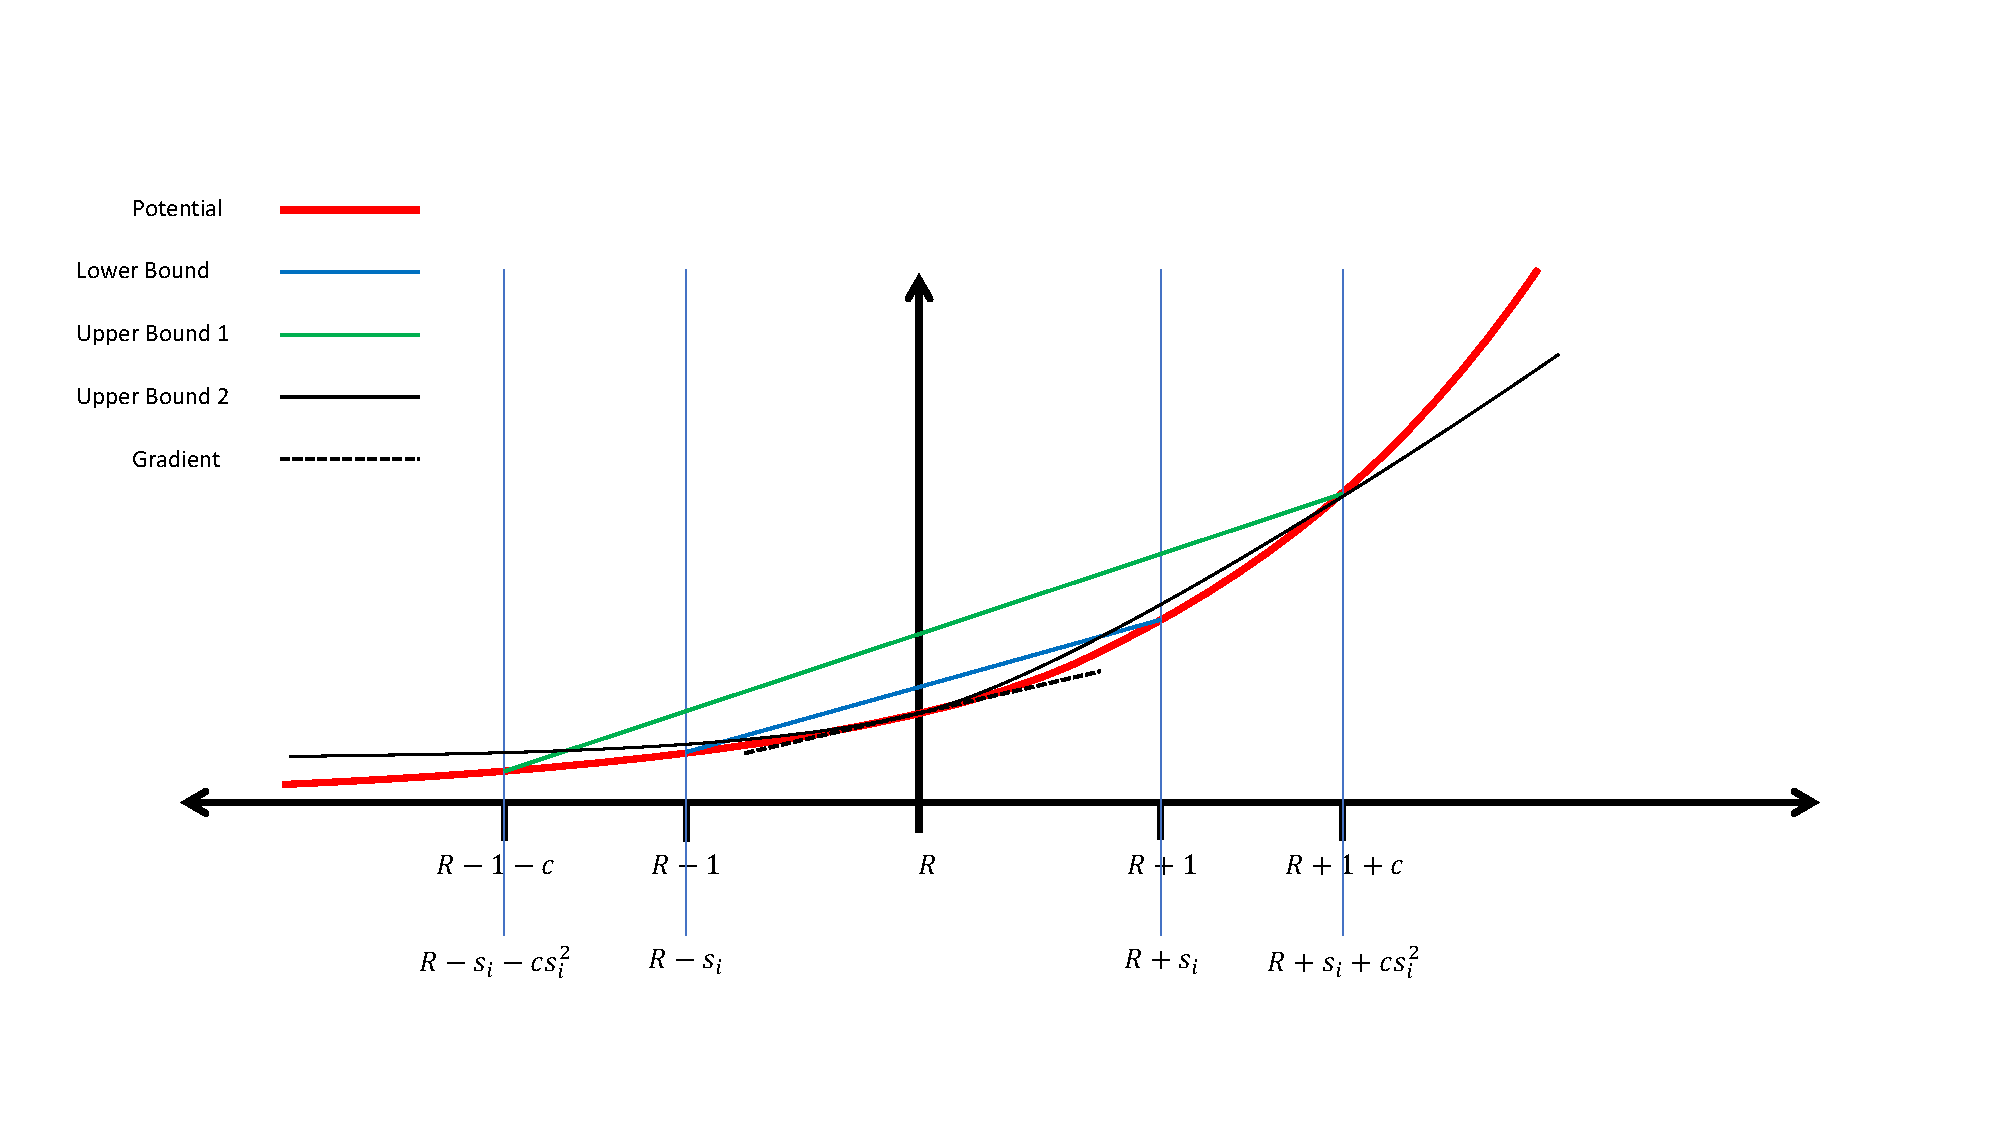
\includegraphics[width=\textwidth]{figures/convexPot.pdf}}
\caption{This figure depicts the relationship between the different
  upper and lower bounds used in the analysis. To aid understanding we
  describe the elements of the figure twice: once for the integer
  game, and once for the continuous time game. \newline
  {\bf Integer time game:} let
  the current iteration be $i$ and let the current regret be $\R$. Let
  $r$ be the regret at iteration $i+1$, we have that $\R-2 \leq r
  \leq \R+2$. The potential at iteration $i+1$ is $\pot(i+1,r)$ (the red curve). The lower bound
  (blue line) corresponds to the adversarial strategy:
  $\adversM^{1/2}(i,\R)$. The first-order learner strategy:
  $\learnerM^1(i,\R)$ corresponds to the green line. The second-order
  learner strategy:  $\learnerM^2(i,\R)$ corresponds to the black
  curve.\newline
{\bf Continuous time game:} let
  the current iteration be $i$, the current time be $t_i$ and the
  current regret be $\R$. Let $0<s_i\leq 1$ be the step size chosen by the
  adversary, so that the next time is $t_{i+1} = t_i+s_i^2$. Let $r$
  be the regret at iteration
  $i+1$, we have that $\R-s_i-c s_i^2 \leq r \leq \R+s_i+c s_i^2$.
  The potential at iteration $i+1$ is $\pot(t_{i+1},r)$ (the red
  curve).  The lower bound (blue line) corresponds to the adversarial
  strategy: $\adversM^{1/2}_{\pm s_i}(t_i,\R)$. The first-order learner strategy:
  $\learnerM^{1c}(t_i,\R)$ corresponds to the green line. The second-order
  learner strategy: $\learnerM^{2c}(i,\R)$ corresponds to the black
  curve.   Observe that when $s_i \to 0$ the ratio $\frac{s_i}{s_i+c
    s_i^2}$ converges to 1, and the upper and gap between the green
  and blue lines converges to zero.\\
\rule[1ex]{6.5in}{0.5pt}}
\label{fig:ConvexPot}
\end{center}
\vskip -0.4in
\end{figure} 

  \subsection{A learner strategy with a variance-dependent bound}

  As shown in Lemma~\ref{lemma:adversary-prefers-extremes}, the
  adversary always prefers mixed strategies that assign zero
  probability for all steps other than $\pm 1$. Suppose, however, that
  the adversary is not worst-case optimal and chooses steps whose
  length is less than one. The following lemma gives a slightly
  different strategy for the learner, which guarantees a tighter bound
  for this case.

  \begin{lemma} \label{lemma:second-order-bound}
      The learner strategy:
      \begin{equation} \label{eqn:learner-strat-2}
      \learnerM^2(i-1,\R) =  \frac{1}{Z}
      \left. \frac{\partial}{\partial r} \right|_{r=\R} \pot(i,r)
      \end{equation}
      Where $Z$ is a normalization factor
      $$Z = \E{\R \sim \state(i)}{\left. \frac{\partial}{\partial r} \right|_{r=\R} \pot(i,r)}$$
      guarantees the following upper potential against any adversarial
      strategy $\adversM$
      \begin{equation} \label{eqn:value-iteration-upper}
        \upperpot(i-1, \R) = \pot(i,\R) + b(i,\R) \E{l \sim \adversM(i,\R)}{l^2}
      \end{equation}
      where $b(i,\R) = \pot(i,\R+2) -\pot(i,\R) - 2 \left. \frac{\partial}{\partial r} \right|_{r=\R} \pot(i,r)$
   \end{lemma}

   \proof
   To Do
   \qed
   
We compare the bound for $\learnerM^2$ to the bound for $\learnerM^1$
given in Lemma~\ref{lemma:first-order-bound}. We find that when the 
adversary is optimal: $\E{l \sim \adversM(t,\R)}{l^2}=1$ then the
bound for $\learnerM^1$ is better than the bound for $\learnerM^2$, on the
other hand, when $\E{l \sim \adversM(t,\R)}{l^2}$ is close to zero,
$\learnerM^2$ is better than $\learnerM^1$.  

\section{From integer to discrete time}
\label{sec:discrete}

We start with motivation for using time that is indexed by real
values rather than the natural numbers. We distinguish between two
notions of time. The first notion of time is a counter that
counts the iterations of the game, we will call this counter the {\em
  iteration counter } and denote it by $i=0,1,\ldots$. The second,
more interesting notion of time is the time that appears in the regret
bounds, we denote this time by $t_i$ where $i$ is the iteration
number. We restrict the time increments $\Delta t_i =t_i-t_{i-1}$ to
the range $0\leq \Delta t_i \leq 1$.  The magnitude of $\deltat_i$
corresponds to the {\em hardness} of iteration $i$. $\deltat_i=0$
corresponds to the case where the losses of all of the strategies are
equal to a common value $-1 \leq a \leq 1$. In this case the aggregate
loss $\ell=a$, the state does not change:
$\state(i-1)=\state(i)$, $\Delta t_i=0$ and the instantanous regret is zero. On the
other hand $\Delta t_i=1$ corresponds to the adversarial strategy
$\adversM^{1/2}(t-1,R)$ (Eqn.~\ref{eqn:adv-strat}) which maximizes the
instantanous regret.

We introduce an additional step to the integer game. Before the
learner makes it's choice, the 
adversary chooses a real number $0 \leq s_i \leq 1$, by doing so, the
adversary commits that all of the instantanous expert lossesat that
step be in the range $[-s_i,s_i]$. The time step is defined to be $\deltat_i =
s_i^2$.

First, note that the adversary in this game is at least as powerful as
the adversary in the integer game. This is because the adversary can
always choose $s_i=1$, effectively reducing the game to the integer
game.

Next, we justify the choice $\deltat_i = s_i^2$. Our argument is that
any significantly different choice would give the game to one side or
the other.  Suppose that $s_i = 1/k$ on all $m_k$ iterations of the game. In
other words, this is a rescaling of the integer game. Consider the
adversarial strategy. The distribution (state) after $m_k$ iterations is the
binomial distribution. with mean zero and variance $m_k \frac{1}{k^2}$
if $m_k \gg \frac{1}{k^2}$ then the variance at the end of the game
goes to infinity.

By allowing $\Delta t_i$ to vary from iteration to iteration
we get a more refined quantification of the regret and, as we show
below, min/max optimality.

To find the relationship between loss magnitude and time increments 
we compare two adversarial strategies.  The first strategy, discussed above,
generates losses $\pm 1$ with equal probability, we deonte this
strategy by $\adversM^{1/2}_{\pm 1}$. The other strategy, denoted
$\adversM^{1/2}_{\pm 1/k}$, generates losses of $\pm 1/k$ with equal
probabilities.

From the adversarial point of view $\adversM^{1/2}_{\pm 1/k}$ is worse
than $\adversM^{1/2}_{\pm 1}$. So it should correspond to a smaller
time increment. But how much smaller? Suppose we start with the
initial state $\state(0)$ which is a delta functions at $\R=0$.  One
iteration of $\adversM^{1/2}_{\pm 1}$ results in a distribution
$\pm 1$ w.p, $(1/2,1/2)$, which has mean $0$ and variance $1$.
Suppose we associate $\Delta t =1/j$ with a single step of
$\adversM^{1/2}_{\pm 1/k}$.  Equivalently, we associate $j$ iterations
of $\adversM^{1/2}_{\pm 1/k}$ with $t=1$.  How should we set $j$? the
distribution generated by $j$ steps is a binomial distribution
supported on $j+1$ points, so there is no hope of making the two
distributions identical. However, as it turns out, it is enough to
equalize the mean and the variance of the two distributions. The mean
of $\adversM^{1/2}_{\pm 1/k}$ is zero for any $k$. As for the
variances, a single iteration of $\adversM^{1/2}_{\pm 1}$ is 1 and a
single iteration of $\adversM^{1/2}_{\pm 1/k}$ is $1/k^2$. It follows
that the variance after $j$ iterations of $\adversM^{1/2}_{\pm 1/k}$
$j/k^2$. Equating this variance with that of a single step of
$\adversM^{1/2}_{\pm 1}$ we get $j=k^2$ and $\Delta t= 1/k^2$.

Note a curious behaviour of the {\em range} of $\R$ as $k \to \infty$
the number of steps increases like $k^2$ while the size of each step
is $1/k$. This means that the range of $\R$ is $[-k,k]$, which becomes
converges to $(-\infty, + \infty)$ when $k \to \infty$. On the other
hand, the variance increases like $t$.

Next lets consider effect of reducing the step size on a {\em biased}
strategy $\adversM^{1/2+\gamma}_{\pm 1}$ as defined in
Eqn~(\ref{eqn:adv-strat-p}) for some
$0\leq \gamma \leq 1/2$.  We now figure out what  $\gamma'$ should be
so that the distribution generated by $k^2$ iterations of $\adversM^{1/2+\gamma'}_{\pm 1/k}$ has the
same mean as a single iteration of $\adversM^{1/2+\gamma}_{\pm
  1}$. The mean of a single iteration of
$\adversM^{1/2+\gamma}_{\pm 1}$ is $2\gamma$ while the mean of a
single iteration of $\adversM^{1/2+\gamma'}_{\pm 1/k}$ is
$2\gamma'/k$. Therefor to keep the means equal we need to set
$2\gamma'/k = 2\gamma$ or $\gamma' = \gamma/k$.


Note that as $k \to \infty$, $\gamma' \to 0$. This observation
motivates scaling the bound on $\ell(t)$ like $c s_i^2$ (see the
description of the game below.)



This leads to the following formulation of a continuous time game.
The game is a generalization of the integer time game in that it
reduces to the integer time game if the adversary always chooses $s_i=1$. 

In this game we use $i=1,2,3,\ldots$ as the iteration index. We use
$t_i$ to indicate a sequence of real-valued time points. $t_0=0$ and
we assume there exists a finite $n$ such that $t_n = T$.

We will later give some particular potential functions for which no
a-priori knowledge of the termination condition is needed. The
associated bounds will hold for any iteration of the game.

\subsection{The discrete time game}
\label{sec:discrete-Time-Game}

On iteration $i=1,2,\ldots$
\begin{enumerate}
\item  If $t_{i-1}=T$ the game terminates.
\item The adversay chooses a {\em step size} $0<s_i\leq 1$, which advances
  time by $t_i = t_{i-1}+s_i^2$.
\item Given $s_i$, the learner chooses a distribution $\learnerM(i)$ over $\reals$.
\item The adversary chooses a mapping from $\reals$ to distributions
  over $[-s_i,+s_i]$: $\adversM(t): \reals \to \Delta^{[-s_i,+s_i]}$
\item The aggregate loss is calculated:
  \begin{equation} \label{eqn:ell-discrete}
    \ell(t_i)=\E{\R \sim \state(t_i)}{\learnerM(t_i,\R)
      \Bias(t_i,\R)},\;\mbox{ where } \Bias(t_i,\R) \doteq \E{y \sim \adversM(t_i,\R)}{y}
  \end{equation}
\item the aggregate loss is restricted $|\ell(t_i)| \leq c s_i^2$.
\item The state is updated. The expectation below is over
  distributions. and the notation $G \oplus \R$ means
  that distribution $G$ over the reals is shifted by the amount
  defined by the scalar $\R$:
  $$\state(t_i) = \E{\R \sim \state(t_{i-1})}{\adversM(t_i)(\R)\oplus (\R-\ell(t_i))}
  $$
\end{enumerate}

When $t_i=T$ the game is terminated, and the final value is calculated:
$$\score(T) =\E{\R \sim \state(T)}{\finalPot(\R)}$$

\subsection{Results for the discrete time game}

In the discrete time game the adversary has an additional choice, the
choice of $s_i$. Thus the adversary's strategy includes that choice.
There are two constraints on this choice: $s_i \geq 0$ and
$\sum_{i=1}^n s_i^2 = T$. Note that even that by setting $s_i$
arbitrarily small, the adversary can make the number of steps - $n$ -
arbitrarily large. We will therefor not identify a single adversarial
strategy but instead consider the supremum over an infinite sequence
of strategies.

We use $N(0,\sigma)$ to denote the normal distribution with mean 0 and
std $\sigma$.

\begin{theorem}
  ~\\

   let $A = \E{\R \sim N(0,\sqrt{T})}{\pot(T,\R)}$
   \begin{itemize}
     \item
    For any $\epsilon>0$ there exists a strategy for the adversary
    such that for any strategy of the learner $\score(T) \geq A-\epsilon$
  \item
    There exists a strategy for the learner that guarantees, against
    any adversary $\score(T) \leq A$.
  \end{itemize}
\end{theorem}


\subsection{The adversary prefers smaller steps} \label{sec:smallsteps}
As noted before, if the adversary chooses $s_i=1$ for all $i$ the game
reduces the the integer time game. The question is whether the
adversary would prefer to stick with $s_i=1$ or instead prefer to use
$s_i<1$. In this section we give a surprising answer to this question
-- the adversary always prefers a smaller value of $s_i$ to a larger
one. This leads to a preference for $s_i \to 0$, as it turns out, this
limit is well defined and corrsponds to Brownian motion, also known as
Wiener process.

Consider a sequence of adversarial strategies $S_k$ indexed by
$k=0,1,2,$. The adversarial strategy $S_k$ is corresponds to always
choosing $s_i = 2^{-k}$, and repeating  $\adversM^{1/2}_{\pm 2^{-k}}$ 
for $T 2^{2k}$ iterations.
This corresponds to the distribution created by a random walk with
$T 2^{2k}$ time steps, each step equal to $+2^{-k}$ or  $-2^{-k}$ with probabilities $1/2,1/2$.
Note that in order to preserve the variance, halving the step size
requires incresing the number of iterations by a factor of four.

Let $\pot(S_k,t,\R)$ be the value associated with adversarial
strategy $S_k$, time $t$ (divisible by $2^{-2k}$) and
location $\R$. We are ready to state our main theorem.

\begin{theorem}\label{thm:smallerSteps}
  If the final value function has a strictly positive fourth
  derivative:
  $$ \frac{d^4}{d \R^4} \finalPot(\R) >0, \forall \R$$
  then for any integer $k>0$ and any $0 \leq  t \leq T$, such that $t$
  is divisible by
  $2^{-2k}$ and any $\R$,
  $$\pot(S_{k+1},t,\R)) >  \pot(S_{k},t,\R)$$
\end{theorem}

Before proving the theorem, we describe it's
consequence for the online learning problem.
We can restrict Theorem~\ref{thm:smallerSteps} for the
case $t=0$,$\R=0$ in which case we get an increasing sequence:
\[
\pot(S_1,0,0) < \pot(S_2,0,0) <\cdots <\pot(S_k,0,0) <
\]
The limit of the strategies $S_k$ as $k \to \infty$ is the well
studied Brownian or Wiener process. The backwards recursion that
defines the value function is the celebrated Backwrds Kolmogorov
Equation with zero dift and unit variance
\begin{equation} \label{eqn:Kolmogorov}
  \frac{\partial}{\partial t} \pot(t,\R)
  + \frac{1}{2} \frac{\partial^2}{\partial \R^2} \pot(t,\R)=0
\end{equation}
Given a final value function with a strictly positive fourth
derivative we can use Equation~(\ref{eqn:Kolmogorov}) to compute the
value function for all $0 \leq t \leq T$. We will do so in he next section.

We now go back to proving Theorem~\ref{thm:smallerSteps}. The core of
the proof is a lemma which compares, essentially, the value recursion
when taking one step of size 1 to four steps of size 1/2.


Consider the advesarial strategies $S_k$ and $S_{k+1}$ at a particular
time point $0 \leq t \leq T$ such that $t$ is divisible by
$\deltat=2^{-2k}$ and at a particular location $\R$. Let
$t'=t+\deltat$, and fix a value
function for time , $\pot(t',\R)$ and compare between
two values at $\R,t$. The first value denoted
$\pot_k(t,\R)$ corresponds to $S_k$, and consists of a single random step of $\pm 2^{-k}$. 
The other value $\pot_{k+1}(t,\R)$ corresponds to $S_{k+1}$ and consists of
four random steps of size $\pm 1/2$.

\begin{lemma} \label{lemma:n-strictly-convex}
If $\pot(t',\R)$ is, as a function of $\R$ continuous, strictly
convex and with a strictly positive fourth derivative. Then
\begin{itemize}
\item $\pot_k(t,\R) < \pot_{k+1}(t,\R)$
  \item Both $\pot_k(t,\R)$ and $\pot_{k+1}(t,\R)$ are continuous, strictly
convex and with a strictly positive fourth derivative.
\end{itemize}
\end{lemma}

\proof
Recall the notations $\deltat = 2^{-2k}$ $t' = t+\deltat$ and $s=2^{-k}$.
We can write out explicit expressions for the two values:
\begin{itemize}
\item For strategy $S_0$ the value is
  $$\pot_k(t, \R) = \frac{\pot(t',\R+s)+ \pot(t',\R-s)}{2} $$.
\item For strategy $S_1$ the value is
  $$\pot_{k+1}(t, \R) = \frac{1}{16}
  \paren{\pot(t',\R+2s)+ 4\pot(t',\R+s)+ 6\pot(t',\R)+  4\pot(t',\R-s)+ \pot(t',\R-2s)}
  $$.
\end{itemize}

We want to show that $\pot_1(T-1,\R) > \pot_0(T-1,\R)$ for all $\R$, in
other words we want to characterize the properties of $\finalPot$ the
would garantee that
\begin{equation}\label{eqn:4thOrderConvex}
\pot_1(t,\R) - \pot_0(t,\R) =
\frac{1}{16}
\paren{ \pot(t',\R+2) - 4\pot(t',\R+1) +6\pot(t',\R) - 4\pot(t',\R-1) +\pot(t',\R-2)} > 0
\end{equation}

Inequalities of this form have been studied extensively under the name
``divided differences''~\cite{popoviciu1965certaines,butt2016generalization, de2005divided}.
A function $\finalPot$ that satisfies
inequality~\ref{eqn:4thOrderConvex} is said to be {\em 4'th order convex}
(see details in in~\cite{butt2016generalization}).

$n$-convex functions have a very simple characterization:
\begin{theorem}
  Let $f$ be a  function with is differentiable up to order $n$, and
  let $f^{(n)}$ denote the $n$'th derivative, then $f$ is $n$-convex
  ($n$-strictly convex) if and only if $f^{(n)} \geq 0$ ($f^{(n)} > 0$).
\end{theorem}

We conclude that if $\pot(t',\R)$ has a strictly positive fourth
derivative then $\pot_{k+1}(t,\R) > \pot_{k}(t,\R)$ for all $\R$, proving
the first part of the lemma.

The second part of the lemma follows from the fact that
both $\pot_{k+1}(t,\R)$ and $\pot_{k}(t,\R)$ are convex combinations of
$\pot(t,\R)$ and therefor retain their continuity and convexity properties.

\qed

\proof  of Theorem~\ref{thm:smallerSteps} \\
The proof is by double induction over $k$ and over $t$.
For a fixed $k$ we take a finite backward induction over
$t=T-2^{-2k},T-2 \times 2^{-2k},T-3 \times 2^{-2k},\cdots,0$.
Our inductive claims are that $\pot_{k+1}(t,\R) > \pot_{k}(t,\R)$ and
$\pot_{k+1}(t,\R)$,$\pot_{k}(t,\R)$ are continuous, strongly convex and
have a strongly positive fourth derivative. That these claims carry over
from $t=T-i \times 2^{-2k}$ to  $t=T-(i+1) \times 2^{-2k}$ follows
directly from Lemma~\ref{lemma:n-strictly-convex}.

The theorem follows by forward induction on $k$.

\qed

\subsection{Strategies for the Learner in the discrete time game}
The strategies we propose for the learner in the discrete time game
are an adaptation of the strategies $\learnerM^1,\learnerM^2$ from the
integer time game to the case where $s_i<1$.

We start with the high-level idea. Consider iteration $i$ of the
continuous time game. We know that the adversary prefers $s_i$ to be
as small as possible. On the other hand, the adversary has to choose
some $s_i>0$. This means that the adversary always plays
sub-optimally. Based on $s_i$ the learner makes a choice and the
adversary makes a choice. As a result the current state $\state(t_{i-1})$
is transformed to $\state(t_i)$. To choose it's strategy, the learner
needs to assign value possible states $\state(t_i)$. How can she do
that? By assuming that in the future the adversary will play
optimally, i.e. setting $s_i$ arbitrarily small. While the adversary
cannot be optimal, it can get arbitrarily close to optimal, which is
brownian motion.

Solving the backwards Kolmogorov equation with the boundary condition
$\pot(T,\R)$ yields $\pot(t,\R)$ for any
$\R \in \reals$ and $t \in [0,T]$. We now explain how using this
potential function we derive strategies for the the learner. 

Note that the learner chooses a distribution {\em after} the adversary
set the value of $s_i$. The discrete time version of $\learnerM^1$
(Eqn~\ref{eqn:learner-strat-1}) is 
\begin{eqnarray} \label{eqn:learner-strat-1c}
  \learnerM^{1d}(t_{i-1},\R) = \frac{1}{Z^{1d}}
  \frac{\pot(t_i,\R+s_{i-1}+cs_{i-1}^2) -
  \pot(t_i,\R-s_{i-1}-cs_{i-1}^2)}{2} \\
  \mbox{ where } Z^{1d} = \E{\R \sim \state(t_i)}{\frac{\pot(t_i,\R+s_{i-1}+cs_{i-1}^2) -
  \pot(t_i,\R-s_{i-1}-cs_{i-1}^2)}{2}} \nonumber
\end{eqnarray}

Next, we consider the discrete time version of $\learnerM^2$:
(Eqn~\ref{eqn:learner-strat-2})
\begin{eqnarray} \label{eqn:learner-strat-2c}
  \learnerM^{2d}(t_{i-1},\R) =  \frac{1}{Z^{2d}}
  \left. \frac{\partial}{\partial r} \right|_{r=\R}
  \pot(t_{i-1}+s_{i-1}^2,r)
  \\
  \mbox{ where } Z^{2d} = \E{\R \sim
  \state(t_i)}{\left. \frac{\partial}{\partial r} \right|_{r=\R} \pot(t_{i-1}+s_{i-1}^2,r)} \nonumber
\end{eqnarray}

\section{Bounds for easy sequences} \label{sec:easy}
In Section~\ref{sec:discrete} we have shown that the integer time game
has a natural extension to a setting where $\deltat_i = s_i^2$. We
also showed that the adversary gains from setting $s_i$ as small as
possible.

We characterized the optimal adversarial strategy for the discrete
time game (Section~\ref{sec:discrete-Time-Game}), which corresponds
to the adversary choosing the loss to be $s_i$ or $-s_i$ with equal
probabilities. A natural question at this point is to characterize the
regret when the adversary is not optimal, or the sequences are ``easy''.

To see that such an improvement is possible, consider the following
{\em constant} adversary. This adversary associates the same loss to
all experts on iteration $i$, formally, $\adversM(i,\R) = l$. In this
case the average loss is also equal to $l$, $\ell(i)=l$ which means
that all of the instantaneous regrets are $r=l-\ell(t_i) = 0$, which,
in turn, implies that $\state(i) = \state(i+1)$. As the state did not
change, it makes sense to set $t_{i+1}=t_i$, rather than
$t_{i+1}=t_i+s_i^2$.

We observe two extremes for the adversarial behaviour. The constant
adversary described above for which $t_{i+1} = t_i$, and the random walk adversary described
earlier, in which each expert is split into two, one half with loss
$-s_i$ and the other with loss $+s_i$. In which case $t_{i+1} =
t_i+s_i^2$ which is the maximal increase in $t$ that the adversary can
guarantee. The analysis below shows that these are two extremes on a
spectrum and that intermediate cases can be characterized using a
variance-like quantity.

We define a variant of the discrete time game
(\ref{sec:discrete-Time-Game}) For concreteness we include the
learner's strategy, which is the limit of the strategy in the discrete
game when $s_i \to 0$.

\subsubsection{The continuous time game and a learner strategy}
\label{sec:contin-Time-Game}
Set $t_1=0$ \\
Fix maximal step $0<s<1$ \\
On iteration $i=1,2,\ldots$

\begin{enumerate}
\item  If $t_i=T$ the game terminates.
\item Given $t_{i-1}$, the learner chooses a distribution
  $\learnerM(i)$ over $\reals$:
  \begin{equation} \label{eqn:learner-strat-cc}
  \learnerM^{cc}(t,\R) =  \frac{1}{Z^{cc}}
  \left. \frac{\partial}{\partial r} \right|_{r=\R} \pot(t,r)
  \mbox{ where } Z^{cc} = \E{\R \sim \state(t_i)}{\left. \frac{\partial}{\partial r} \right|_{r=\R} \pot(t,r)}
\end{equation}

\item The adversay chooses a {\em step size} $0<s_i\leq s$ and a mapping from $\reals$ to distributions
  over $[-s_i,+s_i]$: $\adversM(t): \reals \to \Delta^{[-s_i,+s_i]}$
\item The aggregate loss is calculated:
  \begin{equation} \label{eqn:ell-discrete}
    \ell(t_i)=\E{\R \sim \state(t_i)}{\learnerM^{cc}(t_i,\R)
      \Bias(t_i,\R)},\;\mbox{ where } \Bias(t_i,\R) \doteq \E{y \sim \adversM(t_i,\R)}{y}
  \end{equation}
  the aggregate loss is restricted to $|\ell(t_i)| \leq c s_i^2$.
\item  Increment $t_{i+1} = t_{i} + \deltat_i$ where
\begin{equation} \label{eqn:deltat}
  \deltat_i=
  \E{\R \sim \state(t_i)}{\E{y \sim
      \adversM(t_i,\R)}{\at{\frac{\partial^2}{\partial r^2}}
      ((y-\ell(t_i))^2)}}
\end{equation}

\item The state is updated. The expectation below is over
  distributions. and the notation $G \oplus \R$ means
  that distribution $G$ over the reals is shifted by the amount
  defined by the scalar $\R$:
  $$\state(t_{i+1}) = \E{\R \sim \state(t_{i})}{\adversM(t_i)(\R)\oplus (\R-\ell(t_i))}
  $$
\end{enumerate}

~\\
----------------------------------------------------
~\\

Our characterization applies to the limit where the $s_i$ are small. Formally, we define
\begin{definition}
We say that an instance of the discrete time game is
$(n,s,\tau)$-bounded if it consists of $n$ iterations and $\forall\;\; 0<i\leq n,\;\; s_i < s$ and $\sum_{j=1}^n s_j^2=\tau$
\end{definition}

Note that $\tau>t_n$ and that $\tau$ depends only on the ranges $s_i$
while $t_n$ depends on the variance. $t_n = T$ 
is the dominant term in the regret bound, while $\tau$ controls the
error term.

\begin{theorem} \label{thm:variancebound} Let $\pot \in \SP{\infty}$
  be a potential function that satisfies the Kolmogorov backward
  equation~(\ref{eqn:Kolmogorov}).
  Assume a sequence of $(n_i,s_i,\tau)$-bounded games where $\tau$ is
  a constant $n \to \infty$ and $s = \sqrt{\frac{\tau}{n}}$

Then 
$$\score(\state(t_{i+1})) \leq \score(\state(t_i))+O(s \tau)$$
\end{theorem}

The proof is given in appendix~\ref{appendix:ProofOfVarianceBound}

If we define

\begin{equation} \label{eqn:Vn}
  V_n = t_n = \sum_{i=1}^n \deltat_i= 
  \sum_{i=1}^n \E{\R \sim \state(t_i)}{\E{y \sim \adversM(t_i,R)}{\at{\frac{\partial^2}{\partial r^2}}
      (y-\ell(t_i))^2}} 
\end{equation}

We can use $V_n$ instead of $T$ giving us a variancee based bound.

  
%    \E{\R \sim \state(i-1)}{ \E{y \sim
%      \adversM(i-1)(\R)}{\pot(i,\R+y-\ell(i-1))}}

\section{Two self-consistent potential functions} \label{sec:self-consistent}

The potential functions, $\pot(t,\R)$ is a solution of PDE~(\ref
{eqn:Kolmogorov}):
\begin{equation} 
  \frac{\partial}{\partial t} \pot(t,\R)
  + \frac{1}{2} \frac{\partial^2}{\partial r^2} \pot(t,\R)=0
\end{equation}
under a boundary condition $\pot(T,\R)=\finalPot(\R)$, which we assume
is in $\SP{4}$

So far, we assumed that the game horizon $T$ is known in advance. We
now show two value functions where knowledge of the horizon is not
required. Specifically, we call a value function $\pot(t,\R)$
{\em self consistent} if it is defined for all $t>0$ and if for any
$0<t<T$, setting $\phi(T,\R)$ as the final potential and solving for
the Kolmogorov Backward Equation yields $\phi(t,\R)$ regarless of the
time horizon $T$. 

We consider two solutions to the PDE, the exponential potential and
the NormalHedge potential. We give the form of the potential function
that satisfies Kolmogorov Equation~\ref{eqn:Kolmogorov}, and derive
the regret bound corresponding to it.

{\bf The exponential potential function} which corresponds to exponential
  weights algorithm corresponds to the following equation
\[
    \pot_{\mbox{exp}}(\R,t) = e^{\sqrt{2} \eta \R - \eta^2 t}
  \]
  Where $\eta>0$ is the learning rate parameter.
  
Given $\epsilon$ we choose $\eta = \sqrt{\frac{\ln (1/\epsilon)}{t}}$
we get the regret bound that holds for any $t>0$
  \begin{equation}
    \R_\epsilon \leq \sqrt{2 t \ln \frac{1}{\epsilon}}
  \end{equation}
Note that the algorithm depends on the choice of $\epsilon$, in other
words, the bound does {\em not} hold for all values of $\epsilon$ at
the same time.

{\bf The NormalHedge value} is
\begin{equation} \label{eqn:NormalHedge}
  \pot_{\mbox{NH}}(\R,t) = \begin{cases}
    \frac{1}{\sqrt{t+\nu}}\exp\left(\frac{\R^2}{2(t+\nu)}\right)
    & \mbox{if } \R \geq 0  \\
  \frac{1}{\sqrt{t+\nu}} & \mbox{if } \R <0
  \end{cases}
\end{equation}
Where $\nu>0$ is a small constant. The function $\pot_{\mbox{NH}}(\R,t)$,
restricted to $\R\geq 0$ is in $\SP{4}$ and is a constant for $\R \leq 0$.

The regret bound we get is:
\begin{equation}
\R_\epsilon \leq \sqrt{(t+\nu) \left( \ln (t+\nu) + 2 \ln \frac{1}{\epsilon}\right)}
\end{equation}
This bound is slightly larger than the bound for exponential weights,
however, the NormalHedge bound holds simultanuously for all
$\epsilon>0$ and the algorithm requires no tuning.


\section{NormalHedge yields the fastest increasing potential} \label{sec:NormalHedge}

Up to this point, we considered any continuous value function with
strictly positive derivatives 1-4. We characterized the min-max
strategies for any such function. It is time to ask whether value
functions can be compared and whether there is a ``best'' value
function. In this section we give an informal argument that
NormalHedge is the best function. We hope this argument can be
formalized.

We make two observations. First, the min-max strategy for the
adversary does not depend on the potential function! (as long as it
has strictly positive derivatives). That strategy corresponds to the
brownian process.

Second, the argument used to show that the regret relative to
$\epsilon$-fraction of the expert is based on two arguments
\begin{itemize}
\item The average value function does not increase with time.
\item The (final) value function increases rapidly as a function of $\R$
\end{itemize}
The first item is true by construction. The second argument suggests
the following partial order on value functions. Let
$\pot_1(t,\R),\pot_2(t,\R)$ be two value functions such that
\[
\lim_{\R \to \infty} \frac{\pot_1(t,\R)}{\pot_2(t,\R)} = \infty  
\]
then $\pot_1$ {\em dominates} $\pot_2$, which we denote by, $\pot_1 > \pot_2$.

On the other hand, if the value function increases too quickly, then,
when playing against brownian motion, the average value will increase
without bound.  Recall that the distribution of the brownian process
at time $t$ is the standard normal with mean 0 and variance $t$.
The question becomes what is the fastest the value
function can grow, as a function of $\R$ and still have a finite
expected value with respect to the normal distribution.

The answer seems to be NormalHedge (Eqn.~\ref{eqn:NormalHedge}). More
precisely, if $\epsilon>0$, the mean value is finite, but if
$\epsilon=0$ the mean value becomes infinite.

\bibliographystyle{plain}
\bibliography{ref.bib}

\appendix
\section{Proof of Theorem~\ref{thm:simulBoundAveragePot}}
\proof
  \begin{itemize}
  \item
  {\bf $\state$ satisfies a simultanous bound for $B$ if it satisfies an
  average potential bound for $\pot = B^{-1}$}\\
Assume by contradiction that $\state$ does not satisfy the simultanous bound. In
other words there exists $a \in \reals$ such that
$\P{\R \sim \state}{\R > a} > B(a)$. From Markov inequality and the fact
that $\phi$ is non decreasing we get
\[
  \E{\R \sim \state}{\pot(\R)} \geq \phi(a) \P{\R \sim \state}{\R > a} >
  \phi(a) B(a) = \frac{B(a)}{B(a)}=1
\]
but $ \E{\R \sim \state}{\pot(\R)} >1$ contradicts the average potential
assumption for the potential $\phi(\R) = B(\R)^{-1}$
\item
{\bf $\state$ satisfies an
  average potential bound for $\pot = B^{-1}$ if it satisfies a simultanous bound for $B$}\\
As $\phi$ is a non-decreasing function, and assuming $\R,\R'$ are drawn
independently at random according to $\state$:
\begin{eqnarray}
  \E{\R \sim \state}{\pot(\R)} & = & \E{\R \sim \state}{\pot(\R)
                                  \P{\R' \sim \state}{\phi(R') \geq \phi(\R)}} \\
                            & \leq & \E{\R \sim \state}{\pot(\R)
                                     \P{\R' \sim \state}{R' \geq \R}} \\
                            & < & \E{\R \sim \state}{\pot(\R) B(\R)} \\
                            & = & \E{\R \sim \state}{\frac{B(\R)}{B(\R)}}
                                  = \E{\R \sim \state}{1} = 1
\end{eqnarray}
\end{itemize}
\qed

\section{Proof of Theorem~\ref{thm:variancebound}}
\label{appendix:ProofOfVarianceBound}
We start with two technical lemmas
\begin{lemma} \label{lemma:infiniteexpectations}
Let $f(x) \in \SP{2}$, i.e. $f(x), f'(x),f''(x) >0$ for all $x \in
\reals$, let $h(x)$ be a uniformly bounded function: $\forall x,\;\; |h(x)|<1$.
Let $\state$ be a distribution over $\reals$.
If $\E{x \sim \state}{f(x)}$ is well-defined (and finite) , then 
$\E{x \sim \state}{h(x) f'(x)}$ is well defined (and finite) as well.
\end{lemma}
\proof
Assume by contradiction that $\E{x \sim \state}{h(x) f'(x)}$ is
undefined. Define $h^+(x) = \max(0,h(x))$.
As $f'(x)>0$, this implies that either $\E{x \sim \state}{h^+(x)
  f'(x)}=\infty$ or $\E{x \sim \state}{(-h)^+(x) f'(x)}=\infty$ (or both). 

Assue wlog that $\E{x \sim \state}{h^+(x) f'(x)}=\infty$. As
$f'(x)>0$ and $0 \leq h^+(x) \leq 1$ we get that $\E{x \sim
  \state}{f'(x)}=\infty$.
As $f(x+1) \geq f'(x)$ we get that $\E{x \sim
  \state}{f(x)}=\infty$ which is a contradiction.
\qed

\iffalse
$\epsilon>0$ such that
for any $v>0$ there exists $|h_v(x)| < v$ such that 
$|\E{x \sim \state}{h_v(x) f'(x)}|>\epsilon$. Define $h'_v =
\frac{h_v}{v}$. Clearly $|h'_v(x)|<1$ and we have that
$$|\E{x \sim \state}{h'_v(x) f'(x)}|>\frac{\epsilon}{v}$$

Define the positive parts of $h_v$ to be $h_v^+(x) = \max(0,h'_v(x))$
and $h_v^-(x) = \max(0,-h'_v(x))$. As $f'(x)>0$ we that either
\[
  \E{x \sim \state}{h^+_v(x) f'(x)}>\frac{\epsilon}{v}
\]
or 
\[
  \E{x \sim \state}{h^-_v(x) f'(x)}>\frac{\epsilon}{v}
\]
Wlog assume the first. As $f \in \SP{2}$, we have that $f(x+1) \geq f'(x)$. Therefore
 $\E{x \sim \state}{f(x+1)|h_v^(x)>0)}=\infty$. As $f(x)>0$ for all $x$ we
 find that $\E{x \sim \state}{f(x)}=\infty$ which contradicts the
 Lemma's assumption.
\qed
\fi

\newcommand{\Dx}{\Delta x}
\newcommand{\Dy}{\Delta y}
\begin{lemma} \label{lemma:Taylor2D}
Let $f(x,y)$ be a differentiable function with continuous derivatives
up to degree three. Then
\begin{eqnarray}
  &&f(x_0+\Dx,y_0+\Dy) = f(x_0,y_0)
  + \atI{\frac{\partial}{\partial x}} \Dx 
  + \atI{\frac{\partial}{\partial y}} \Dy \\
  &+&\frac{1}{2} \atI{\frac{\partial^2}{\partial x^2}} \Dx^2
      +\atI{\frac{\partial^2}{\partial x\partial y}} \Dx\Dy
      +\frac{1}{2} \atI{\frac{\partial^2}{\partial y^2}} \Dy^2\\
  &+&\frac{1}{6} \atII{\frac{\partial^3}{\partial x^3}} \Dx^3
      +\frac{1}{2} \atII{\frac{\partial^3}{\partial x^2 \partial y}} \Dx^2\Dy\\
  &&+ \frac{1}{2} \atII{\frac{\partial^3}{\partial x \partial y^2}} \Dx\Dy^2
    + \frac{1}{6} \atII{\frac{\partial^3}{\partial y^3}} \Dy^3
\end{eqnarray}
for some $0\leq t \leq 1$.
\end{lemma}
\proof {\em of Lemma~\ref{lemma:Taylor2D}} 
Let $F:[0,1] \to \reals$ be defined as  $F(t)=f(x(t),y(t))$ where
$x(t) = x_0+t\Dx$ and $y(t)=y_0+t\Dy$. Then $F(0)=f(x_0,y_0)$ and
$F(1)=f(x_0+\Dx,y_0+\Dy)$. It is easy to verify that
$$ \frac{d}{dt}F(t)
=\frac{\partial}{\partial x} f(x(t),y(t))\Dx
+ \frac{\partial}{\partial y} f(x(t),y(t))\Dy
$$
and that in general:
\begin{equation} \label{eqn:d.dn.F}
\frac{d^n}{d t^n} F(t) = \sum_{m=1}^n {n \choose m}
\frac{\partial^n}{\partial x^m \partial y^{n-m}} f(x_0+t \Dx,y_0+t\Dy)
\Dx^m \Dy^{n-m}
\end{equation}
As $f$ has partial derivatives up to degree 3, so does $F$. Using the
Taylor expansion of $F$ and the intermediate point theorem we get that
\begin{equation} \label{eqn:Taylor.F}
  f(x_0+\Dx,y_0+\Dy) = F(1) = F(0)+\frac{d}{dt}F(0)
  +\frac{1}{2}\frac{d^2}{dt^2}F(0)
  +\frac{1}{6}\frac{d^3}{dt^3}F(t')
\end{equation}
Where $0 \leq t' \leq 1$. Using Eqn~(\ref{eqn:d.dn.F}) to expand each
term in Eqn.~(\ref{eqn:Taylor.F}) completes the proof.
\qed


\proof {\em of Theorem~\ref{thm:variancebound}}\\
We prove the claim by an upper bound on the increase of potential that holds for any iteration $1 \leq i \leq n$:
\begin{equation} \label{proof:onestep}
\score(\state(t_{i+1})) \leq \score(\state(t_i)) + a s_i^3 \mbox{ for some constant } a>0
\end{equation}
Summing inequality~(\ref{proof:onestep}) over all iterations we get that 
\begin{equation} \label{proof:allsteps}
\score(\state(T)) \leq \score(\state(0)) + c \sum_{i=1}^n s_i^3 \leq 
\score(\state(0)) + a s \sum_{i=1}^n s_i^2 = 
\score(\state(0)) + a s T
\end{equation}
From which the statement of the theorem follows.

We now prove inequality~(\ref{proof:onestep}). 
We use the notation $r=y -\ell(i)$ to denote the instantaneous regret at iteration $i$. 


Applying Lemma~\ref{lemma:Taylor2D} to
$\pot(t_{i+1},\R_{i+1})=\pot(t_i+\deltat_i,\R_i+r_i)$  we get
\begin{eqnarray} 
    \pot(t_i+\deltat_i,\R_i+r_i) & =&  
    \pot(t_i,\R_i)\\
    &+&\at{\frac{\partial}{\partial \rho}} r_i \\
    &+&\at{\frac{\partial}{\partial \tau}}  \deltat_i \\
    &+& \frac{1}{2} \at{\frac{\partial^2}{\partial \rho^2}} r_i^2 \\
    &+& \at{\frac{\partial^2}{\partial r \partial \tau}} r_i \deltat_i \label{term:Taylor_rdt}\\
    &+& \frac{1}{2} \at{\frac{\partial^2}{\partial \tau^2}} \deltat_i^2 \label{term:Taylor_dtsquare}\\
    &+& \frac{1}{6} \att{\frac{\partial^3}{\partial \rho^3}} r_i^3 \label{term:Taylor_r3}\\
    &+& \frac{1}{2} \att{\frac{\partial^3}{\partial \rho^2 \partial \tau}} r_i^2\deltat_i \label{term:Taylor_r2t}\\
    &+& \frac{1}{2} \att{\frac{\partial^3}{\partial \rho \partial \tau^2}} r_i\deltat_i^2 \label{term:Taylor_rt2}\\
    &+& \frac{1}{6} \att{\frac{\partial^3}{\partial \tau^3}} \deltat_i^3 \label{term:Taylor_t3}
\end{eqnarray}
for some $0 \leq g \leq 1$.

By assumption $\pot$ satisfies the Kolmogorov backward equation:
\begin{equation*} 
  \frac{\partial}{\partial \tau} \pot(\tau,\rho)
  = -\frac{1}{2} \frac{\partial^2}{\partial r^2} \pot(\tau,\rho)
\end{equation*}
Combining this equation with the exchangability of the order of
partial derivative (Clairiaut's Theorem) we can substitute all
partial derivatives with respect to $\tau$ with partial derivatives
with respect to $\rho$ using the following equation.
\[
  \frac{\partial^{n+m}}{\partial \rho^n \partial \tau^m} \pot(\tau,\rho)=
  (-1)^m \frac{\partial^{n+2m}}{\partial \rho^{n+2m}} \pot(\tau,\rho)
\]
Which yields
\begin{eqnarray}
      \pot(t_i+\deltat_i,\R_i+r_i) & =&  
    \pot(t_i,\R_i)\\
    &+& \at{\frac{\partial}{\partial \rho}} r_i \label{term:coll1}\\
    &+& \at{\frac{\partial^2}{\partial \rho^2}} \paren{\frac{r_i^2}{2}-\deltat_i} \label{term:coll2}\\
    &-& \at{\frac{\partial^3}{\partial \rho^3}} r_i \deltat_i \label{term:coll3}\\
    &+& \frac{1}{2} \at{\frac{\partial^4}{\partial \rho^4}} \deltat_i^2 \label{term:coll4}\\
    &+& \frac{1}{6} \att{\frac{\partial^3}{\partial \rho^3}} r_i^3 \label{term:coll5}\\
    &-& \frac{1}{2} \att{\frac{\partial^4}{\partial \rho^4}} r_i^2\deltat_i \label{term:coll6}\\
    &+& \frac{1}{2} \att{\frac{\partial^5}{\partial \rho^5}} r_i\deltat_i^2 \label{term:coll7}\\
    &-& \frac{1}{6} \att{\frac{\partial^6}{\partial \rho^6}} \deltat_i^3 \label{term:coll8}
\end{eqnarray}

  From the assumption that the game is $(n,s,T)$-bounded we get that 
  \begin{enumerate}
  \item $|r_i| \leq s_i +c s_i^2 \leq 2 s_i$
  \item $\deltat_i \leq s_i^2 \leq s^2$
    % \item $\sum_i \deltat_i=T$
  \end{enumerate}

  given these inequalities we can rewrite the second factor in each
  term as follows, where $|h_i(\cdot)|\leq 1$
  \begin{itemize}
  \item {\bf For~(\ref{term:coll1}):}
    $r_i=2s_i\frac{r_i}{2s_i}=2s_ih_1(r_i)$.
  \item {\bf For~(\ref{term:coll2}):}
    $r_i^2 - \frac{1}{2}\deltat_i = 4s_i^2\frac{r_i^2 -
      \frac{1}{2}\deltat_i}{4s_i^2} = 4s_i^2 h_2(r_i,\deltat_i)$
  \item {\bf For~(\ref{term:coll3}):} $r_i \deltat_i = 2s_i^3
    \frac{r_i \deltat_i}{2s_i^3} = 2s_i^3 h_3(r_i,\deltat_i)$
  \item {\bf For~(\ref{term:coll4}):} $\deltat_i^2 =
    s_i^4\frac{\deltat_i^2}{s_i^4} = s_i^3 h_4(\deltat_i)$
  \item {\bf For~(\ref{term:coll5}):} $r_i^3 = 8s_i^3
    \frac{r_i^3}{8s_i^3} = 8s_i^3 h_5(r_i,\deltat_i)$
  \item {\bf For~(\ref{term:coll6}):} $r_i^2 \deltat_i = 4s_i^4
    \frac{r_i^2 \deltat_i}{4s_i^4} = 4s_i^3 h_6(r_i,\deltat_i)$
  \item {\bf For~(\ref{term:coll7}):} $r_i \deltat_i^2 = 2s_i^5
    \frac{r_i \deltat_i^2}{2s_i^5}$
  \item {\bf For~(\ref{term:coll8}):} $\deltat_i^3 = s_i^6 \frac{\deltat_i^3}{s_i^6}$
\end{itemize}
  We therefor get the simplified equation
  
  \begin{eqnarray*} 
     \pot(t_i+\deltat_i,\R_i+r_i) & =&  \pot(t,\R)+\at{\frac{\partial}{\partial r}} r
    + \at{\frac{\partial}{\partial t}} \deltat \\
                                  &+& 
                                      \frac{1}{2}  \at{\frac{\partial^2}{\partial r^2}} r^2\\
                                  &+& \at{\frac{\partial^2}{\partial r \partial t}} r_i \deltat_i \label{term:Taylor_collected_rdt}\\
                                  &+& \frac{1}{6} \at{\frac{\partial^3}{\partial r^3}} r_i^3 \label{term:Taylor_collected_r3}
                                      + O(s^4)
\end{eqnarray*}

and therefor
  \begin{eqnarray} 
     \pot(t_i+\deltat_i,\R+r) &=& \pot(t_i,\R) +
                                  \at{\frac{\partial}{\partial r}} r
                                  \nonumber \\
    &+& \at{\frac{\partial^2}{\partial r^2}} (r^2 - \deltat_i) +
        O(s^3) \label{eqn:Taylor}
\end{eqnarray}

Our next step is to consider the expected value of~(\ref{eqn:Taylor}) wrt $\R \sim \state(t_i)$,
$y \sim \adversM(t_i,\R)$ for an arbitrary adversarial strategy
$\adversM$.

We will show that the expected potential does not increase:
\begin{equation} \label{eqn:deltatislargeenough}
     \E{\R \sim \state(t_i)}{ \E{y \sim \adversM(t_i,\R)}{\pot(t_i+\deltat_i,\R+y-\ell(t_i))}} \leq \E{\R \sim \state(t_i)}{\pot(t_i,\R)}
\end{equation}

Plugging Eqn~(\ref{eqn:Taylor}) into the LHS of
Eqn~(\ref{eqn:deltatislargeenough}) we get
\begin{eqnarray}
  \lefteqn{\E{\R \sim \state(t_i)}{\E{y \sim \adversM(t_i,\R)}{\pot(t_i+\deltat_i,\R+y-\ell(t_i))}}} \\
  &=& \E{\R \sim \state(t_i)}{\pot(t_i,\R)} \label{eqn:contin0}\\
  &+& \E{\R \sim \state(t_i)}{\E{y \sim \adversM(t_i,\R)}{\at{\frac{\partial}{\partial r}} (y-\ell(t_i))}} \label{eqn:contin1}\\
  &+& \E{\R \sim \state(t_i)}{\E{y \sim
      \adversM(t_i,\R)}{\at{\frac{\partial^2}{\partial r^2}}
      ((y-\ell(t_i))^2 - \deltat_i)}}
  \label{eqn:contin2}\\
  &+& O(s^3) \label{eqn:contin3}
\end{eqnarray}
Some care is needed here. we need to show that the expected value
are all finite. We assume that the expected potential
(Eqn~({eqn:contin0}) is finite. Using
Lemma~\ref{lemma:infiniteexpectations} this implies that the expected
value of higher derivatives of $\frac{\partial}{\partial \R} \pot(\R)$
are also finite.\footnote{I need to clean this up and find an argument
  that the expected value for mixed derivatives is also finite.}


To prove inequality~(\ref{proof:onestep}), we need to show that the
terms~\ref{eqn:contin1} and \ref{eqn:contin2} are smaller or equal to
zero.
~\\~\\~\\
{\bf Term~(\ref{eqn:contin1}) is equal to zero:}\\
As $\ell(t_i)$ is a constant
relative to $\R$ and $y$, and $\at{\frac{\partial}{\partial r}}$ is a
constant with respect to $y$ we can rewrite~(\ref{eqn:contin1}) as
\begin{equation} \label{eqnterm1.1}
  \E{\R \sim \state(t_i)}{\at{\frac{\partial}{\partial r}}
    \E{y \sim \adversM(t_i,\R)}{y} }
- \ell(t_i) \E{\R \sim \state(t_i)}{\at{\frac{\partial}{\partial r}}}
\end{equation}

Combining the definitions of $\ell(t)$~(\ref{eqn:ell-discrete}) and~
and the learner's strategy
$\learnerM^{cc}$~(\ref{eqn:learner-strat-cc}) we get that
\begin{eqnarray}
\ell(t_i) &=& \E{\R \sim \state{t_i}}{\frac{1}{Z}
              \at{\frac{\partial}{\partial r}}
              \E{y \sim \adversM(i,\R)}{y}} \mbox{ where }
              Z=\E{\R \sim \state{t_i}}{\frac{1}{Z}
              \at{\frac{\partial}{\partial r}}}
              \label{eqnterm1.2}
\end{eqnarray}

Plugging~(\ref{eqnterm1.2}) into (\ref{eqnterm1.1}) and recalling the
requirement that $\ell(t_i)<\infty$ we find that
term~(\ref{eqn:contin1}) is equal to zero.


~\\~\\~\\
{\bf Term~(\ref{eqn:contin2}) is equal to zero:}\\
As $\deltat_i$ is a constant relative to $y$, we can take it
outside the expectation and plug in the definition of $\deltat_i$ (\ref{eqn:deltat})
\begin{equation} \label{eqn:term2.1}
  \E{\R \sim \state(t_i)}{\E{y \sim
      \adversM(t_i,\R)}{\adversM(t_i,\R)}{\at{\frac{\partial^2}{\partial r^2}}
      (y-\ell(t_i))^2} - \deltat_i}=
  \deltat_i - \deltat_i =0
\end{equation}
Where $G(t_i,\R)$ is defined in Equation~(\ref{eqn:SecondOrderDerivative})
We find that (\ref{eqn:contin2}) is zero.

Finally (\ref{eqn:contin3}) is negligible relative to the other terms
as $s \to 0$.
\qed 

\end{document}


\iffalse
\begin{definition}[Continuous Time]
The continuous time limit is a sequence of games indexed by
$j=0,1,\ldots$. Suppose the stopping time for all games is equal to
$T$.
Let $s_i^j$ be the step size associated with the
$i'th$ iteration of game $j$. Then $s_i^j$ are supposed to have the
following properties:
\begin{itemize}
\item Let $s^j = \max_i s_i^j$, then $\lim_{j \to \infty} s^j = 0$
  \item for any $j$, $\sum_i (s_i^j)^2 = T$
\end{itemize}
  \end{definition}

\section{Old Stuff}





\section{Variable time steps}
The second order bounds of~\cite{cesa2007improved} show that, in some
contexts, the time parameter $t$ can be replaced by a variance-type
parameter $\V_T= \sum_{i=1}^T \var_i$. This corresponds to a
significant tightening of the bound. For example if instead of $l_j^i
\in [-\epsilon,+\epsilon]$, then $\V_T = T\epsilon^2$, and if we set
$T=\epsilon^{-2}$ we get n upper bound on the regret that does not
depend on $T$. The idea is to replace $T$ with $V_T$ in the definition
of the upper and lower potentials. Which is what we do in
Section\ref{sec:discrete}.

In that variant of the potential game the adversary chooses the
``real-time'' step at each iteration. Surprisingly, it turns out that
the adversary's preference is to make the time steps as small as
possible (but not zero). Combining the random walk strategy with the
infinitesimal time step, we arrive at a strategy that is define by
Brownian motion, or a Wiener process. Even more surprisingly, the
strategy of the learning at this limit corresponds to the same
Brownian motion. In other words, we have a min-max characterization of
DTOL.

\paragraph*{The rest of the paper is organized as follows}
In Section~\ref{sec:preliminaries} we provide some basic definitions.
In Section~\ref{sec:integer} we describe the potential game in the standard
integer time case and prove some upper and lower bounds for this
case. In Section~\ref{sec:discrete} we define a the discrete time
game, where time advances are real valued and finite. The core of our
argument, which is based on the theory of ``divided-differences''
appears in Section~\ref{sec:smallsteps}. In
Section~\ref{sec:continuous} we define the continuous time limit of
the game. In Section~\ref{sec:self-consistent} we show that optimal
any-time potential functions correspond to the solution of the
kolmogorov Backwards differential equation, and show the Exponential weights and
NormalHedge are solutions for that Equation. Finally, in
Section~\ref{sec:NormalHedge}
we argue that NormalHedge is the best possible potential function.

  \fi

  \iffalse
\subsubsection*{Our Contributions}
\begin{itemize}
\item We characterize the min/max strategies for 
  potential functions that have strictly positive derivatives up to
  order four.
\item We show that the optimal adversarial strategy for all of
  these potential functions is a strategy corresponding to
  Brownian motion.
\item We show that $V_T$ replaces $T$ for any of these games.
\item  We show that all potential functions that satisfy a particular
  partial differential equations yield min/max solutions to the
  potential game.
\item We show that both the exponential weights algorithm and
  NormalHedge are solutions to the PDE.
  \item We show that NormalHedge provides the best possible regret bounds.
\end{itemize}

In this paper we extend and refine the analysis of the potential
function to
provide a min/max analysis for a large set of potential functions. We
then show that NormalHedge is, in a strong sense the best of those
potential functions.

Our analysis is based on three ideas that are listed below.
\begin{itemize}
    \item {\bf Potential games:} We focus on the potential function, rather than on the problem of minimizing regret. In other words, we define a new game, in which the goal of the learner is to minimize  the final average potential.
    \item {\bf Experts as a probability space:} Instead of restricting the game to $N$ strategies, we allow the set of strategies to be an arbitrary probability space. This allows the adversary the following simple but powerful strategy.  At each iteration $i$ the adversary splits each one of the strategies into two equal parts, once part incurs loss $-1$ and the other loss $+1$. In other words, at iteration $i$ there are $2^i$ strategies, each corresponding to a sequence in $\{-1,+1\}^i$. It is intuitively clear that the instantaneous loss of the learner is always zero, regardless of it's choice of $P$.
    \item {\bf Reducing the time step and continuous time:} Regret bounds of the form $C\sqrt{T \ln N}$ are tight for the case in which the adversary assigns losses of $\pm 1$ with equal probabilities.
    Suppose however, that the adversary produces the exact same sequence of losses, but divides the range of each loss by 2. In this case the losses and the regrets will all be divided by two, but the bound will remain the same! This suggest that defining $T$ as the number of iterations in the game leaves some slack. To remedy this situation we let time take on real values such that $t_{i+1}-t_i \leq 1$. At the same time we 
    allow the adversary to declare, before each iteration, the range $[-s_i,+s_i]$ for the losses, in which case the following time would be 
    $t_{i+1}=t_i +s_i^2$. Surprisingly, we find out that for a large set of potential functions, the preference of the adversary is to make $s_i$ as small as possible, making iterative game into a continuous time game and the adversarial strategy to be Brownian motion.
\end{itemize}

\fi
